\documentclass[a4paper,oneside,DIV=10,12pt]{scrartcl}

\usepackage{fontspec}
\setmainfont{STIX Two Text}
\setsansfont{Roboto}
\setmonofont{PT Mono}

\usepackage{amsmath}
\usepackage{unicode-math}
\setmathfont{STIX Two Math}

\usepackage{microtype}

\usepackage{polyglossia}
\setmainlanguage{ukrainian}

\usepackage{graphicx}
\usepackage{subcaption}
\usepackage{booktabs}

\usepackage{enumitem,calc}
\DeclareDocumentEnvironment{steps}%
{O{}}% If no argument is given the label defaults to 'Step'
{\begin{enumerate}[leftmargin = *]}% Tune labelindent to set hanging step number
{\end{enumerate}}

\newcommand\barneg[1]{\overline{#1}}

\begin{document}
	\begin{titlepage}
	\begin{center}
		Міністерство освіти і науки України\\
		Національний авіаційний університет\\
		Навчально-науковий інститут комп'ютерних інформаційних технологій\\
		Кафедра комп'ютеризованих систем управління

		\vspace{\fill}
		Лабораторна робота №3\\
		з дисципліни «Комп'ютерна схемотехніка»\\
		на тему «Дослідження елементів і тригерів»\\
		
		\vspace{\fill}
		\begin{flushright}
		Виконав:\\
		студент ННІКІТ СП-225\\
		Клокун Владислав\\
		Перевірив:\\
		Іскренко~Ю.~Ю.
		\end{flushright}
		
		Київ 2017
	\end{center}
	\end{titlepage}
	
	\section{Мета роботи}
		\begin{steps}
			\item Вивчення принципів побудови і логіки роботи тригерів ЕОМ на інтегральних мікросхемах.
			\item Вивчення методів синтезу тригерів ЕОМ.
			\item Вивчення основних методик дослідження асинхронних і синхронних тригерів у статичному і динамічному режимах.
			\item Визначення основних параметрів тригерів ЕОМ.
			\item Ознайомлення з тригерами в серіях мікросхем.
		\end{steps}
	
	\section{Короткі теоретичні відомості}
		\subsection{Визначення та призначення тригерів}
			Тригер — це запам'ятовуючий елемент з двома стійкими станами, зміна яких відбувається під дією вхідних сигналів. Як елемент комп'ютера, тригер призначений для зберігання одного біта інформації, тобто логічного 0 або логічної 1. Схема тригера забезпечує запис, зчитування, стирання та індикацію двійкової інформації, яка зберігається. На основі тригерів будують типові функціональні вузли комп'ютерів — регістри, лічильники, накопичувальні суматори, а також мікропрограмні автомати.
			
			Усі різновиди тригерів являють собою елементарний автомат, який містить власне елемент пам'яті (ЕП) та схему керування (СхК), яка утворює вхідну логіку (рис.~\ref{fig:flipflop-structure-scheme}).
			
			\begin{figure}[!htbp]
			\centering
				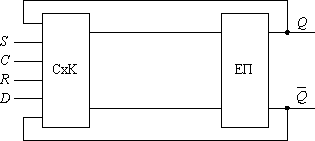
\includegraphics[]{flipflop-structure-scheme.png}
			\caption{Структура тригера у вигляді елемента пам'яті і схеми компонентів}
			\label{fig:flipflop-structure-scheme}
			\end{figure}
			
			Стан тригера визначається сигналами на прямому~$Q$ та інверсному~$\barneg{Q}$ виходах. При позитивному кодуванні інформації високий рівень напруги на прямому виході позначає значення логічної 1 (стан $Q = 1$), а низький рівень~— значення логічного 0 (стан $Q = 0$).
			
			Зміна стану тригера (його перемикання) забезпечується зовнішніми сигналами і сигналами зворотного зв’язку на виході тригера, які поступають на входи схеми керування. Звичайно зовнішні сигнали, як і входи тригера, позначають латинськими буквами R, S, Т, С, V та іншими. В найпростіших схемах тригерів окрема СхК може бути відсутньою. Оскільки функціональні властивості тригерів визначаються їх схемою керування, то назви основних входів переносяться на всю схему тригера.
			
		\subsection{Класифікація тригерів}
			Тригери класифікують за такими ознаками:
			\begin{enumerate}
				\item Логікою функціонування.
				\item Способом запису інформації.
				\item Моментом реакції на тактовий сигнал.
				\item Кількістю тактів синхронізації.
				\item Кількістю ступенів.
				\item Складом логічних елементів.
			\end{enumerate}
			
			\subsubsection{За логікою функціонування}
				Відповідно до логіки функціонування розрізняють такі тригери:
				\begin{enumerate}
					\item З роздільною установкою станів «0» і «1» (RS-тригери).
					\item З одним інформаційним входом (D-тригери).
					\item З лічильним входом (T-тригери).
					\item Універсальні з роздільною установкою станів «0» і «1».
					\item Комбіновані (RST-, RSJK-тригери).
					\item Зі складною вхідною логікою.
				\end{enumerate}
				
				Входи тригерів розділяються на інформаційні (R, S, Т та ін.) та керуючі (С, V). Інформаційні (логічні) входи призначені для прийому сигналів інформації, яка запам'ятовується. Назви вхідних сигналів ототожнюють з назвами входів тригера. Керуючі входи служать для керування записуванням інформації. У тригерах може бути два види керуючих сигналів: синхронізуючий (тактовий) сигнал С, який надходить до С-входу (тактового входу) і дозволяючий сигнал V, який надходить до V-входу.
			
			\subsubsection{За способом запису інформації}
				За способом записування (приймання) інформації розрізняють асинхронні та синхронні (тактовні) тригери. Тригери, які не мають С-входу, називаються асинхронними. В асинхронних тригерах записування інформації відбувається в будь-який момент часу при надходженні сигналів до інформаційних входів.
				
				Тригери, які мають С-вхід, називаються синхронними. У синхронному тригері запис інформації можливий при однакових сигналах на інформаційному і синхронному входах. Цим пояснюється вища стійкість до перешкод синхронних тригерів порівняно з асинхронними.
				
				До V-входів тригера надходять сигнали, які дозволяють ($V = 1$) або забороняють ($V = 0$) записування інформації. У синхронних тригерах з V-входом запис інформації можливий при однакових сигналах на інформаційному, С- і V-входах.
			
			\subsubsection{За кількістю тактів синхронізації}
				Залежно від кількості тактових сигналів, необхідних для формування нового стану, розрізняють однотактові, двотактові та багатотактові тригери.
			
			\subsubsection{За моментом реакції на тактовий сигнал}
				За способом керування записуванням (моментом реакції на тактовий сигнал) виділяють синхронні тригери зі статичним (за рівнем), динамічним (за фронтами) та двоступеневим керуванням. В асинхронних тригерах записування нуля і одиниці можливе у будь-який момент часу, при цьому вхідний інформаційний сигнал одночасно є і керуючим. У синхронних тригерах з керуванням за рівнем записування інформації можливе тільки впродовж тривалості тактового сигналу. При цьому тактові сигнали можуть бути прямими (змінюватися від нуля до одиниці) або інверсними (змінюватися від одиниці до нуля).
				
				При керуванні фронтами дозвіл на записування інформації дається тільки в момент перепаду тактового сигналу від нуля до одиниці (прямий динамічний вхід) або від одиниці до нуля (інверсний динамічний вхід). В інші моменти часу тригер не реагує на вхідні інформаційні сигнали незалежно від рівня тактового імпульсу.
				
			\begin{figure}[!htbp]
			\centering
				\begin{subfigure}[t]{0.2\textwidth}
				\centering
					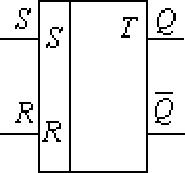
\includegraphics[]{flipflop-rs.pdf}
				\caption{RS-тригер}
				\end{subfigure}
				~
				\begin{subfigure}[t]{0.2\textwidth}
				\centering
					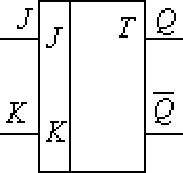
\includegraphics[]{flipflop-jk.pdf}
				\caption{JK-тригер}
				\end{subfigure}
				%
				%\vspace*{\floatsep}
				%
				~
				\begin{subfigure}[t]{0.2\textwidth}
				\centering
					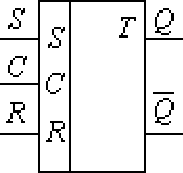
\includegraphics[]{flipflop-rs-sync.pdf}
				\caption{Синхронний RS-тригер}
				\end{subfigure}
				~
				\begin{subfigure}[t]{0.2\textwidth}
				\centering
					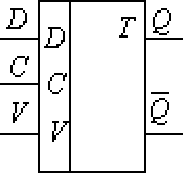
\includegraphics[]{flipflop-d.pdf}
				\caption{D-тригер}
				\end{subfigure}
			\caption{Умовні позначення тригерів}
			\label{fig:flipflop-notation}
			\end{figure}
			
	\section{Хід роботи}
		\subsection{Дослідження роботи асинхронного RS-тригера з інверсними входами на елементах «І—НЕ»}
			Досліджуємо асинхронний RS-тригер з інверсними входами на елементах «І—НЕ».
			
			\begin{figure}[!htbp]
			\centering
				\begin{subfigure}[t]{0.45\textwidth}
				\centering
				\vspace{0pt}
					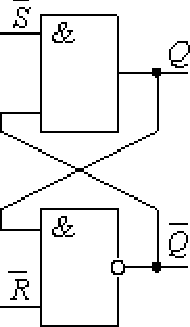
\includegraphics[height=40mm]{assets/03-pdf/flipflop-rs-and-not-schematic.pdf}
				\caption{Схема}
				\label{fig:flipflop-rs-and-not-schematic}
				\end{subfigure}
				~
				\begin{subfigure}[t]{0.45\textwidth}
				\centering
				\vspace{0pt}
					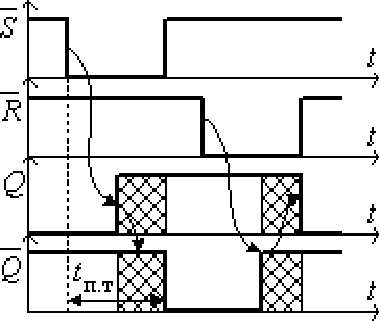
\includegraphics[height=40mm]{assets/03-pdf/flipflop-rs-time-diagram.pdf}
				\caption{Часова діаграма}
				\label{fig:flipflop-rs-time-diagram}
				\end{subfigure}
			\caption{Асинхронний RS-тригер на елементах «І—НЕ»}
			\label{fig:flipflop-rs-and-not}
			\end{figure}
			
			
			
			\begin{steps}
				\item Складаємо схему тригера за рис.~\ref{fig:flipflop-rs-and-not-schematic}.
			
				\item Підключаємо входи $\barneg{R}$ і $\barneg{S}$ до гнізд тумблерного регістра, а входи $Q$ і $\barneg{Q}$ — до світлових індикаторів.
				
				\item Досліджуємо логіку роботи тригера згідно з табл.~\ref{tab:flipflop-rs-inv-excitation-table}, задаючи значення сигналів $\barneg{R}$ і $\barneg{S}$ з тумблерного регістра.
				
				\item Досліджуємо динамічний режим роботи RS-тригера. Для переключення тригера в стан «1» слід подати сигнали від'ємної полярності основної серії CI1 на вхід $\barneg{S}$. Для переключення тригера в стан «0» слід подати сигнали від'ємної полярності допоміжної серії~CI2, затриманої на половину періоду щодо основної серії, на вхід $\barneg{R}$. Замальовуємо осцилограми та вимірюємо час перемикання тригера $t_{\text{П.Т.}}$ (інтервал часу між спадами сигналів на вході~$\barneg{S}$ і~виході~$\barneg{Q}$) за рис.~\ref{fig:flipflop-rs-time-diagram}.
			\end{steps}
			
			\begin{table}[!htbp]
			\centering
				\begin{tabular}{ccc}
					\toprule
						$R_1$ & $S_1$ & $Q_{t+1}$\\
					\midrule
						1     & 1     & $Q_t$\\
						1     & 0     & 1\\
						0     & 0     & — \\
						0     & 1     & 0\\
					\bottomrule
				\end{tabular}
			\caption{Скорочена таблиця переходів асинхронного RS-тригера з інверсними входами}
			\label{tab:flipflop-rs-inv-excitation-table}
			\end{table}
		
		\subsection{Дослідження синхронного RS-тригера з прямими входами на елементах «І—НЕ»}
			Досліджуємо синхронний RS-тригер з прямими входами на елементах «І—НЕ».
			\begin{steps}
				\item Складаємо схему тригера за рис.~\ref{}.
				
				\item Підключаємо входи $R$ і $S$ до гнізд тумблерного регістра, а входи $Q$ і $\barneg{Q}$ — до світлових індикаторів.
				
				\item Досліджуємо логіку роботи тригера згідно з табл.~\ref{tab:flipflop-rs-excitation-table}, задаючи значення сигналів $R$ і $S$ з тумблерного регістра при $C = 1$ (імпульс додатної полярності з виходу ГОІ) після натискання кнопки ПУСК.
				
				\item Досліджуємо динамічний режим роботи синхронного RS-тригера. Для переключення тригера в стан «1» слід подати сигнали додатної полярності основної серії CI1 на вхід $S$ і через схему АБО на вхід $C$. Для переключення тригера в стан «0» слід подати сигнали додатної полярності допоміжної серії~CI2 на вхід $R$ і через схему АБО~— на вхід~$C$. Замальовуємо осцилограми та вимірюємо час перемикання тригера $t_{\text{П.Т.}}$ (інтервал часу між спадами сигналів на вході~$\barneg{S}$ і~виході $\barneg{Q}$) за рис.~\ref{}.
			\end{steps}
			
			\begin{table}[!htbp]
			\centering
				\begin{tabular}{cccc}
					\toprule
						$C$ & $R_1$ & $S_1$ & $Q_{t+1}$\\
					\midrule
						 1  & 0     & 0     & $Q_t$\\
						 1  & 0     & 1     & 1\\
						 1  & 1     & 0     & 0\\
						 1  & 1     & 1     & —\\
						 0  & x     & x     & $Q_t$\\
					\bottomrule
				\end{tabular}
			\caption{Скорочена таблиця переходів синхронного RS-тригера з інверсними входами}
			\label{tab:flipflop-rs-excitation-table}
			\end{table}
		
		\subsection{Дослідження двоступеневого синхронного JK-тригера на елементах «І—НЕ»}
			Досліджуємо двоступеневий синхронний JK-тригер на елементах «І—НЕ».
			\begin{steps}
				\item Складаємо схему за рис.~\ref{}.
				
				\item Досліджуємо логіку роботи тригера згідно з табл.~\ref{tab:jk-flipflop-excitation-table}, задаючи значення сигналів $J$ і $K$ з тумблерного регістра при $C = 1$.
				
				\item Досліджуємо динамічний режим роботи синхронного JK-тригера. Подаємо імпульси додатної полярності CI1 на входи~$J$, $K$ і~$C$. Замальовуємо осцилограми сигналів на виходах~$Q$ і~$\barneg{Q}$ щодо вхідних імпульсів.
			\end{steps}
			
			\begin{table}[!htbp]
			\centering
					\begin{tabular}{cccc}
					\toprule
						$C$ & $J$ & $K$ & $Q_{t + 1}$\\
					\midrule
						1 & 0 & 0 & $Q_{t}$\\
						1 & 0 & 1 & 0\\
						1 & 1 & 0 & 1\\
						1 & 1 & 1 & $\barneg{Q_{t}}$\\
						0 & x & x & $Q_{t}$\\
					\bottomrule
				\end{tabular}
			\caption{Скорочена таблиця переходів синхронного JK-тригера}
			\label{tab:jk-flipflop-excitation-table}
			\end{table}
		
		\subsection{Дослідження D-тригера на елементах «І—НЕ»}
			Досліджуємо D-тригер на елементах «І—НЕ».
			\begin{steps}
				\item Складаємо схему тригерів за рис.~\ref{}.
				
				\item Досліджуємо логіку роботи тригера згідно з табл.~\ref{tab:d-flipflop-excitation-table}, задаючи значення сигналів з тумблерного регістра при $C = 1$.
				
				\item Досліджуємо динамічний режим роботи D-тригера. Підключаємо вхід~$C$ до рівня «1». Подаємо на вхід~$D$ додатні імпульси серії CI1. Замальовуємо осцилограми вхідних і вихідних сигналів і визначаємо час переключення D-тригера.
				\item Досліджуємо динамічний режим роботи D-тригера. Підключаємо вхід~$C$ до рівня «1». Подаємо на вхід~$D$ додатні імпульси серії CI1. Замальовуємо осцилограми вхідних і вихідних сигналів і визначаємо час переключення D-тригера.
			\end{steps}
			
			\begin{table}[!htbp]
			\centering
				\begin{tabular}{ccc}
					\toprule
						$C$ & $D_1$ & $Q_{t + 1}$\\
					\midrule
						1 & 0 & 0\\
						1 & 1 & 1\\
						0 & X & $Q_{t}$\\
					\bottomrule
				\end{tabular}
			\caption{Скорочена таблиця переходів D-тригера}
			\label{tab:d-flipflop-excitation-table}
			\end{table}
		
		
		\subsection{Дослідження D-тригера з динамічним керуванням}
			Досліджуємо D-тригер з динамічним керуванням («схема трьох тригерів»).
			\begin{steps}
				\item Складаємо схему тригера за рис.~\ref{}.
				
				\item Досліджуємо логіку роботи D-тригера згідно з табл.~\ref{tab:d-flipflop-dynamic-excitation-table}. Для цього задаємо значення сигналів $D$ з тумблерного регістра при $C = 1$.
				
				\item Досліджуємо динамічний режим D-тригера за його роботи як лічильного T-тригера. З'єднуємо вихід~$Q$ з інформаційним входом~$D$. Подаємо додатні сигнали серії CI1 на вхід~$C$ (він відіграє роль входу~$T$). Замальовуємо осцилограми вхідних і вихідних сигналів і визначаємо час переключення.
			\end{steps}
			
			\begin{table}[!htbp]
			\centering
				\begin{tabular}{ccc}
					\toprule
						$C$ & $D_1$ & $Q_{t + 1}$\\
					\midrule
						1 & 0 & 0\\
						1 & 1 & 1\\
						0 & X & $Q_{t}$\\
					\bottomrule
				\end{tabular}
			\caption{Скорочена таблиця переходів D-тригера з динамічним керуванням}
			\label{tab:d-flipflop-dynamic-excitation-table}
			\end{table}
			
\end{document}